 \documentclass[border=5pt]{standalone}
     \usepackage[svgnames]{xcolor}
   
    \usepackage{tikz}
    \usetikzlibrary{matrix,decorations.pathreplacing, calc, positioning,fit}
    \usepackage{amsmath}
    \usepackage{mathtools}
 
    \begin{document}

    
   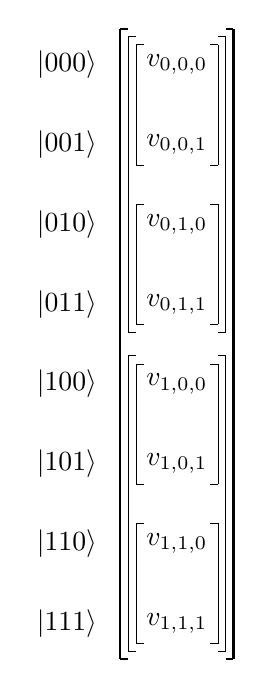
\begin{tikzpicture}[>=stealth,thick,baseline]
    \matrix [matrix of math nodes, row sep=1.5em, column sep=1.5em,](A){ 
    v_{0,0,0} \\
    v_{0,0,1} \\
    v_{0,1,0} \\
	v_{0,1,1} \\
	v_{1,0,0} \\
	v_{1,0,1} \\
	v_{1,1,0} \\ 
    v_{1,1,1} \\
    };
    

%	\draw (A-1-1.north west){}+(-0.1,+0.1) -- (A-1-1){}+(2,0);

	\draw[]  ($(A-1-1.north west) + (-0.2,+0.2)$) -- ($(A-8-1.south west) + (-0.2,-0.2)$);
	\draw[]  ($(A-1-1.north west) + (-0.2,+0.2)$) -- ++(0.1,0);
	\draw[]  ($(A-8-1.south west) + (-0.2,-0.2)$) -- ++(0.1,0); 	

	\draw[]  ($(A-1-1.north east) + (+0.2,+0.2)$) -- ($(A-8-1.south east) + (+0.2,-0.2)$);
	\draw[]  ($(A-1-1.north east) + (+0.2,+0.2)$) -- ++(-0.1,0);
	\draw[]  ($(A-8-1.south east) + (+0.2,-0.2)$) -- ++(-0.1,0); 	


	\draw[thin]  ($(A-1-1.north west) + (-0.1,+0.1)$) -- ($(A-4-1.south west) + (-0.1,-0.1)$);
	\draw[thin]  ($(A-1-1.north west) + (-0.1,+0.1)$) -- ++(0.1,0);
	\draw[thin]  ($(A-4-1.south west) + (-0.1,-0.1)$) -- ++(0.1,0);

	\draw[thin]  ($(A-5-1.north west) + (-0.1,+0.1)$) -- ($(A-8-1.south west) + (-0.1,-0.1)$);
	\draw[thin]  ($(A-5-1.north west) + (-0.1,+0.1)$) -- ++(0.1,0);
	\draw[thin]  ($(A-8-1.south west) + (-0.1,-0.1)$) -- ++(0.1,0);


	\draw[thin]  ($(A-1-1.north east) + (+0.1,+0.1)$) -- ($(A-4-1.south east) + (+0.1,-0.1)$);
	\draw[thin]  ($(A-1-1.north east) + (+0.1,+0.1)$) -- ++(-0.1,0);
	\draw[thin]  ($(A-4-1.south east) + (+0.1,-0.1)$) -- ++(-0.1,0);

	\draw[thin]  ($(A-5-1.north east) + (+0.1,+0.1)$) -- ($(A-8-1.south east) + (+0.1,-0.1)$);
	\draw[thin]  ($(A-5-1.north east) + (+0.1,+0.1)$) -- ++(-0.1,0);
	\draw[thin]  ($(A-8-1.south east) + (+0.1,-0.1)$) -- ++(-0.1,0);




	\draw[ultra thin]  (A-1-1.north west) -- ++(0.1,0);
	\draw[ultra thin]  (A-1-1.north west) -- 
	                   (A-2-1.south west);
	\draw[ultra thin]  (A-2-1.south west) -- ++(0.1,0);	
	
	\draw[ultra thin]  (A-1-1.north east) -- ++(-0.1,0);
	\draw[ultra thin]  (A-1-1.north east) -- 
	                   (A-2-1.south east);
	\draw[ultra thin]  (A-2-1.south east) -- ++(-0.1,0);	
	
	\draw[ultra thin]  (A-3-1.north west) -- ++(0.1,0);
	\draw[ultra thin]  (A-3-1.north west) -- 
	                   (A-4-1.south west);
	\draw[ultra thin]  (A-4-1.south west) -- ++(0.1,0);	
	
	\draw[ultra thin]  (A-3-1.north east) -- ++(-0.1,0);
	\draw[ultra thin]  (A-3-1.north east) -- 
	                   (A-4-1.south east);
	\draw[ultra thin]  (A-4-1.south east) -- ++(-0.1,0);	
	
	\draw[ultra thin]  (A-5-1.north west) -- ++(0.1,0);
	\draw[ultra thin]  (A-5-1.north west) -- 
	                   (A-6-1.south west);
	\draw[ultra thin]  (A-6-1.south west) -- ++(0.1,0);	
	
	\draw[ultra thin]  (A-5-1.north east) -- ++(-0.1,0);
	\draw[ultra thin]  (A-5-1.north east) -- 
	                   (A-6-1.south east);
	\draw[ultra thin]  (A-6-1.south east) -- ++(-0.1,0);	
	
	\draw[ultra thin]  (A-7-1.north west) -- ++(0.1,0);
	\draw[ultra thin]  (A-7-1.north west) -- 
	                   (A-8-1.south west);
	\draw[ultra thin]  (A-8-1.south west) -- ++(0.1,0);	
	
	\draw[ultra thin]  (A-7-1.north east) -- ++(-0.1,0);
	\draw[ultra thin]  (A-7-1.north east) -- 
	                   (A-8-1.south east);
	\draw[ultra thin]  (A-8-1.south east) -- ++(-0.1,0);	


   \node[
     fit=(A-1-1)(A-1-1),
     inner xsep=10pt,inner ysep=5pt,
     label=left: $|000\rangle$
    ](K00) {};

   \node[
     fit=(A-2-1)(A-2-1),
     inner xsep=10pt,inner ysep=5pt,
     label=left: $|001\rangle$
    ](K01) {};


   \node[
     fit=(A-3-1)(A-3-1),
     inner xsep=10pt,inner ysep=5pt,
     label=left: $|010\rangle$
    ](K10) {};


   \node[
     fit=(A-4-1)(A-4-1),
     inner xsep=10pt,inner ysep=5pt,
     label=left: $|011\rangle$
    ](K11) {};


   \node[
     fit=(A-5-1)(A-5-1),
     inner xsep=10pt,inner ysep=5pt,
     label=left: $|100\rangle$
    ](K00) {};

   \node[
     fit=(A-6-1)(A-6-1),
     inner xsep=10pt,inner ysep=5pt,
     label=left: $|101\rangle$
    ](K01) {};


   \node[
     fit=(A-7-1)(A-7-1),
     inner xsep=10pt,inner ysep=5pt,
     label=left: $|110\rangle$
    ](K10) {};


   \node[
     fit=(A-8-1)(A-8-1),
     inner xsep=10pt,inner ysep=5pt,
     label=left: $|111\rangle$
    ](K11) {};

%   \node[
%     fit=(A-6-4)(A-6-4),
%     inner xsep=20pt,inner ysep=20pt,
%     label=below: $j$-ième colonne
%     ](C) {};
%
%    \draw[->](L.east)-- (A-4-4);
%    \draw[->](C.south)-- (A-4-4);

    \end{tikzpicture}

    
    
\end{document}
    
    
    